%%---------------------------------------------------------------------------%%
\section{Results}
\label{sec:results}

In this section we describe briefly some selected results related to the flow in the full core and the cases described in Section~\ref{sec:model}.

\subsection{Full core simulations and FOM update}
\label{sec:results1}

The first we examine is Case I which is the largest at $59.8 10^{9}$ unique grid points. This is the case used to determine updated FOMs for the CFD component of ExaSMR. The layer size and time step $dt=3 \cdot 10^{-4}$ are consistent with previous calculation performed.  This simulation campaign corresponds effectively to a strong scaling study for the full core mesh ranging from 40\% to 100\% of Summit.

Details of the strong scaling study are provided in Figure illustrating the time per time step as the simulation progresses and the overall wall time. An average time per time-step is determined as an average between 100 and 200 time steps. We note that for the previous FOM calculation this number was determined between 50 and 100 steps. However this difference is likely has a  minimal effect on the overall FOM, as the time per time-step does not change in average significantly after 50 steps.

\begin{figure}[!ht]
\centering
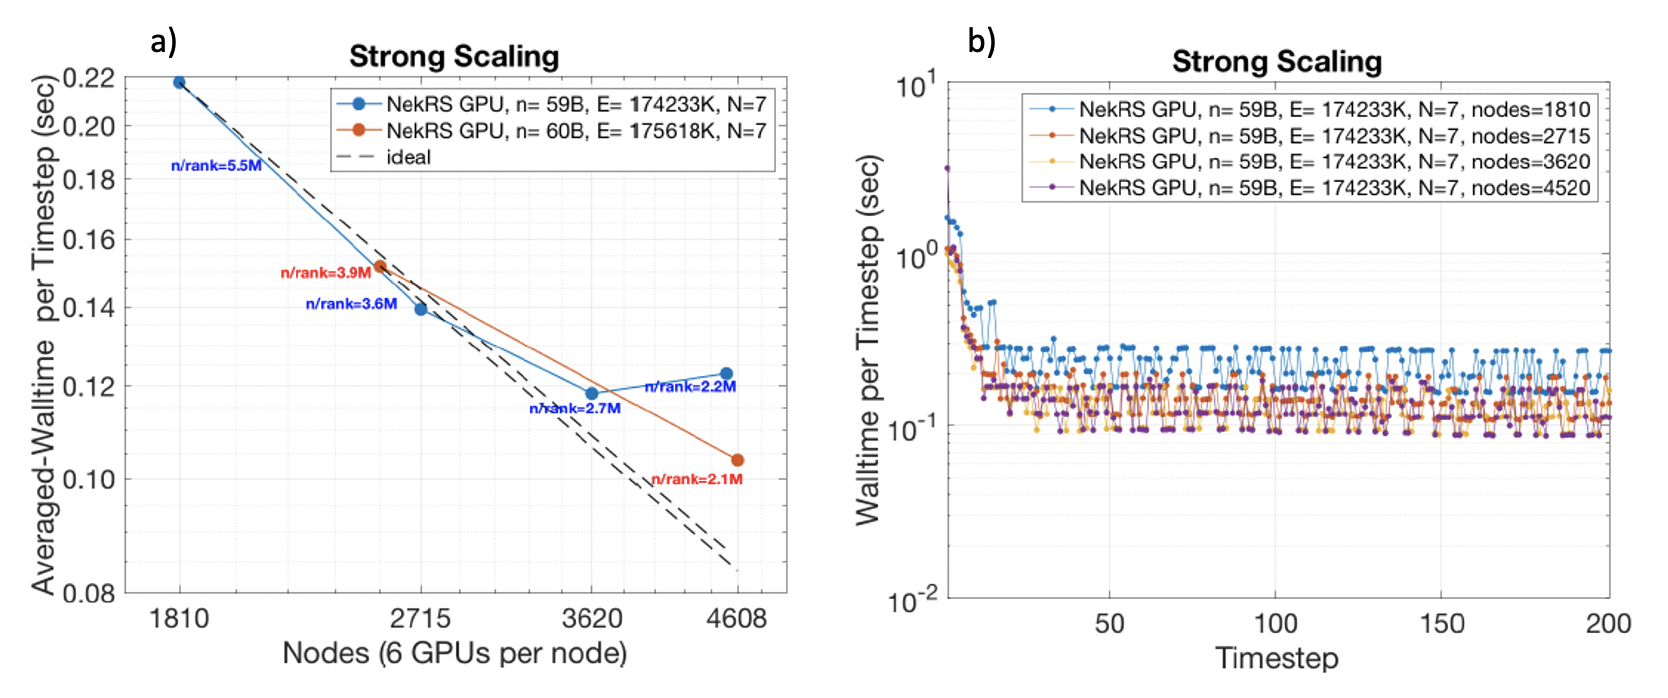
\includegraphics[width=0.9\textwidth]{./figures/full_core_strong.png}
\caption{Full core strong scaling study. a) average wall time per step. b) time per time step as simulation progresses. }
\label{fig:strong}
\end{figure}

The data collected has been used to generated updated FOM measurements in Table~\ref{tab:FOM}. This table includes both the measured FOM and the projected FOM to full machine for each of the cases. The cases with lower number of nodes should be considered a more accurate representation of full core projections for larger cases. The higher node counts are clearly below the strong scaling limit and likely do not have a sufficient number of element per GPU.

We note that the FOM measured is significantly higher than the previous projected measurement on Summit: $1.44 \cdot 10^{11}$ dofs/s. The value reported show a 4.9x increase in projected values. We also note that the performance now is orders of magnitude higher than the FOM measured on Titan in 2018.

% Full core: n= 5.9762e+10 = E*N^3,          Previous 30M:  before (dofs/s)= 1.44506e+11
% node  rank   E                E/gpu  N  nstep  dt           cfl       t_step     avg_t_step       n/t_step     n/avg_t_step          1.44506e+11/(n/t_step)     1.44506e+11/(n/avg_t_step)
%4525  27150  174233000  6417   7  100    3.0e-04  0.58    9.34e-02   1.22e-01      6.3985e+11   4.8985e+11           4.4278e+00                      3.3898e+00
%4608  27648  174233000  6301   7  100    3.0e-04  0.58    9.01e-02   1.21e-01      6.6328e+11   4.9390e+11

 \begin{table} \centering \small
  % \resizebox{0.48\textwidth}{!}{
   \begin{tabular}{cccccc} \hline \hline
    Nodes & $E$/GPU & Fraction of machine & Average Time per step [s] & FOM (dofs/s) & Projected FOM (dofs/s) \\ \hline
    1810 & 	16043 & 0.393 &	0.2175  & $2.75 \cdot 10^{11}$ & $7.00 \cdot 10^{11}$ \\
    2715 &	10695 & 0.589 &	0.1395  & $4.29 \cdot 10^{11}$ & $7.28 \cdot 10^{11}$ \\
    3620 &	8021 & 0.786 &	0.1182  & $5.06 \cdot 10^{11}$ & $6.44 \cdot 10^{11}$ \\
    4525 &	6417 & 0.981 &	0.1229  & $4.87 \cdot 10^{11}$ & $4.95 \cdot 10^{11}$ \\
    4608 &	6301 & 1.000 &	0.121   & $4.94 \cdot 10^{11}$ & $4.94 \cdot 10^{11}$ \\
     \hline \hline
  \end{tabular}
   \caption{FOM measurement based on full core mesh. $E=174233000$, $N=7$.}
   \label{tab:FOM}
  \end{table}

\subsection{RANS full core simulations}
\label{sec:results2}

\begin{figure}[!ht]
\centering
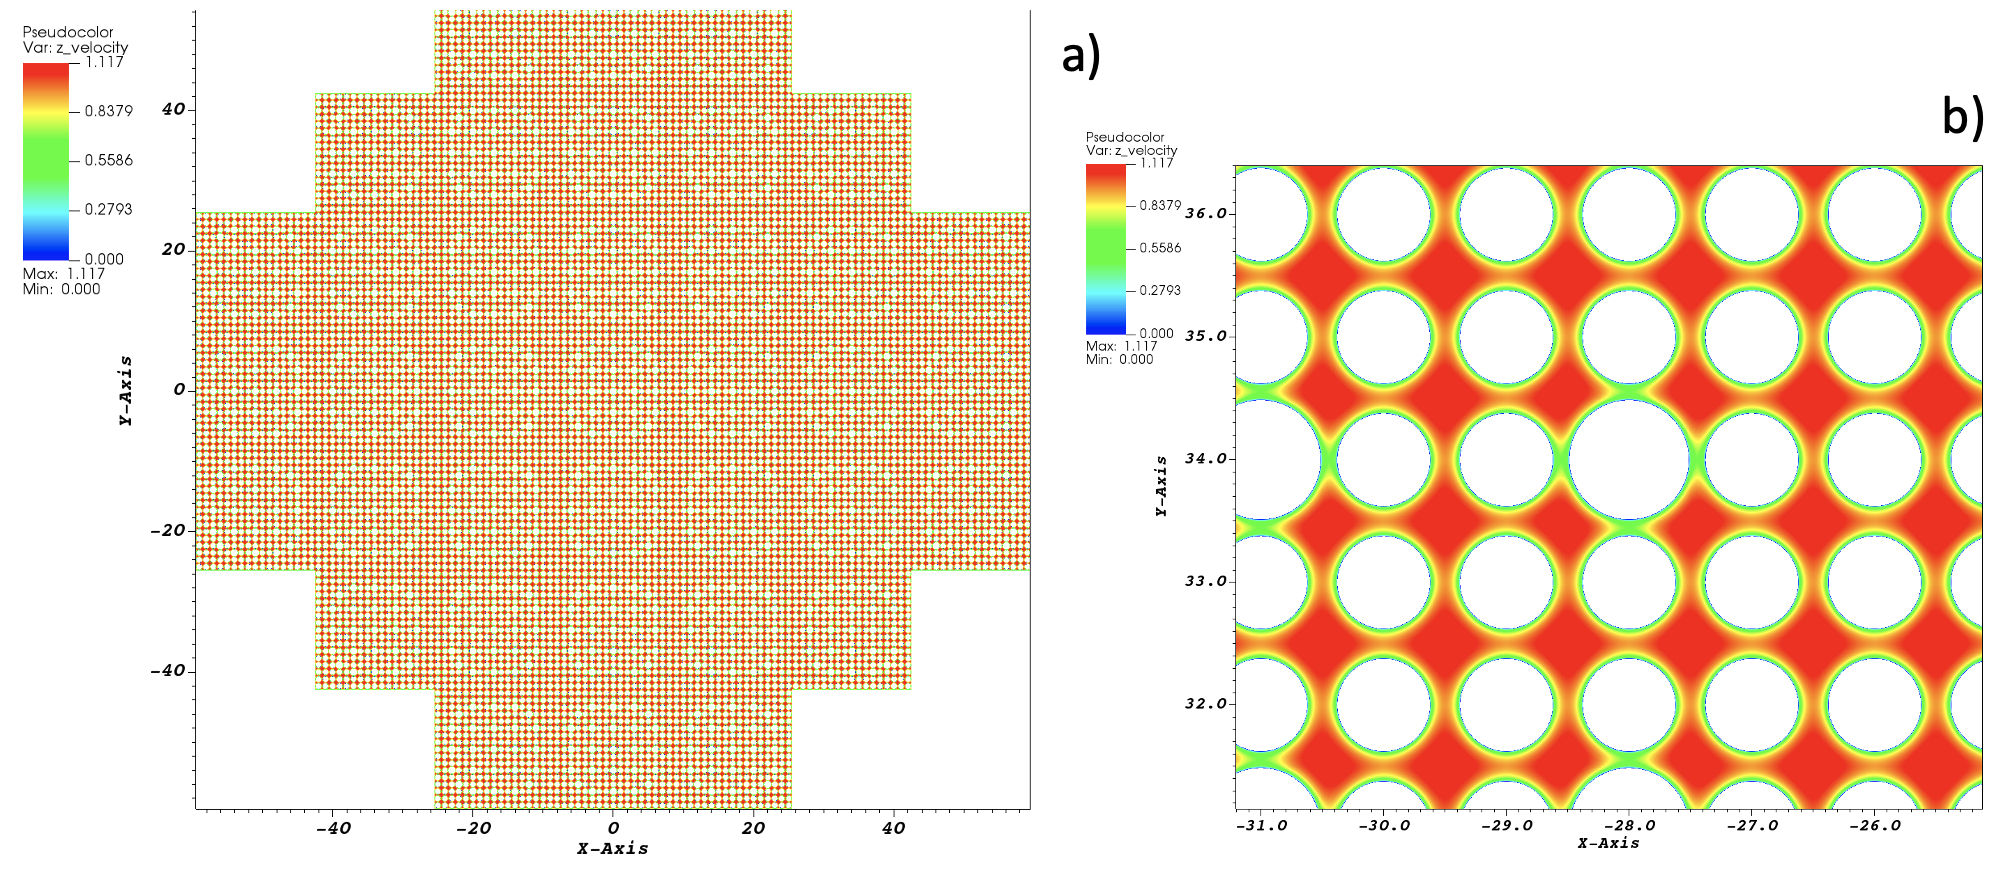
\includegraphics[width=0.9\textwidth]{./figures/periodic_vz.png}
\caption{Cross section of}
\label{fig:vz}
\end{figure}

\begin{figure}[!ht]
\centering
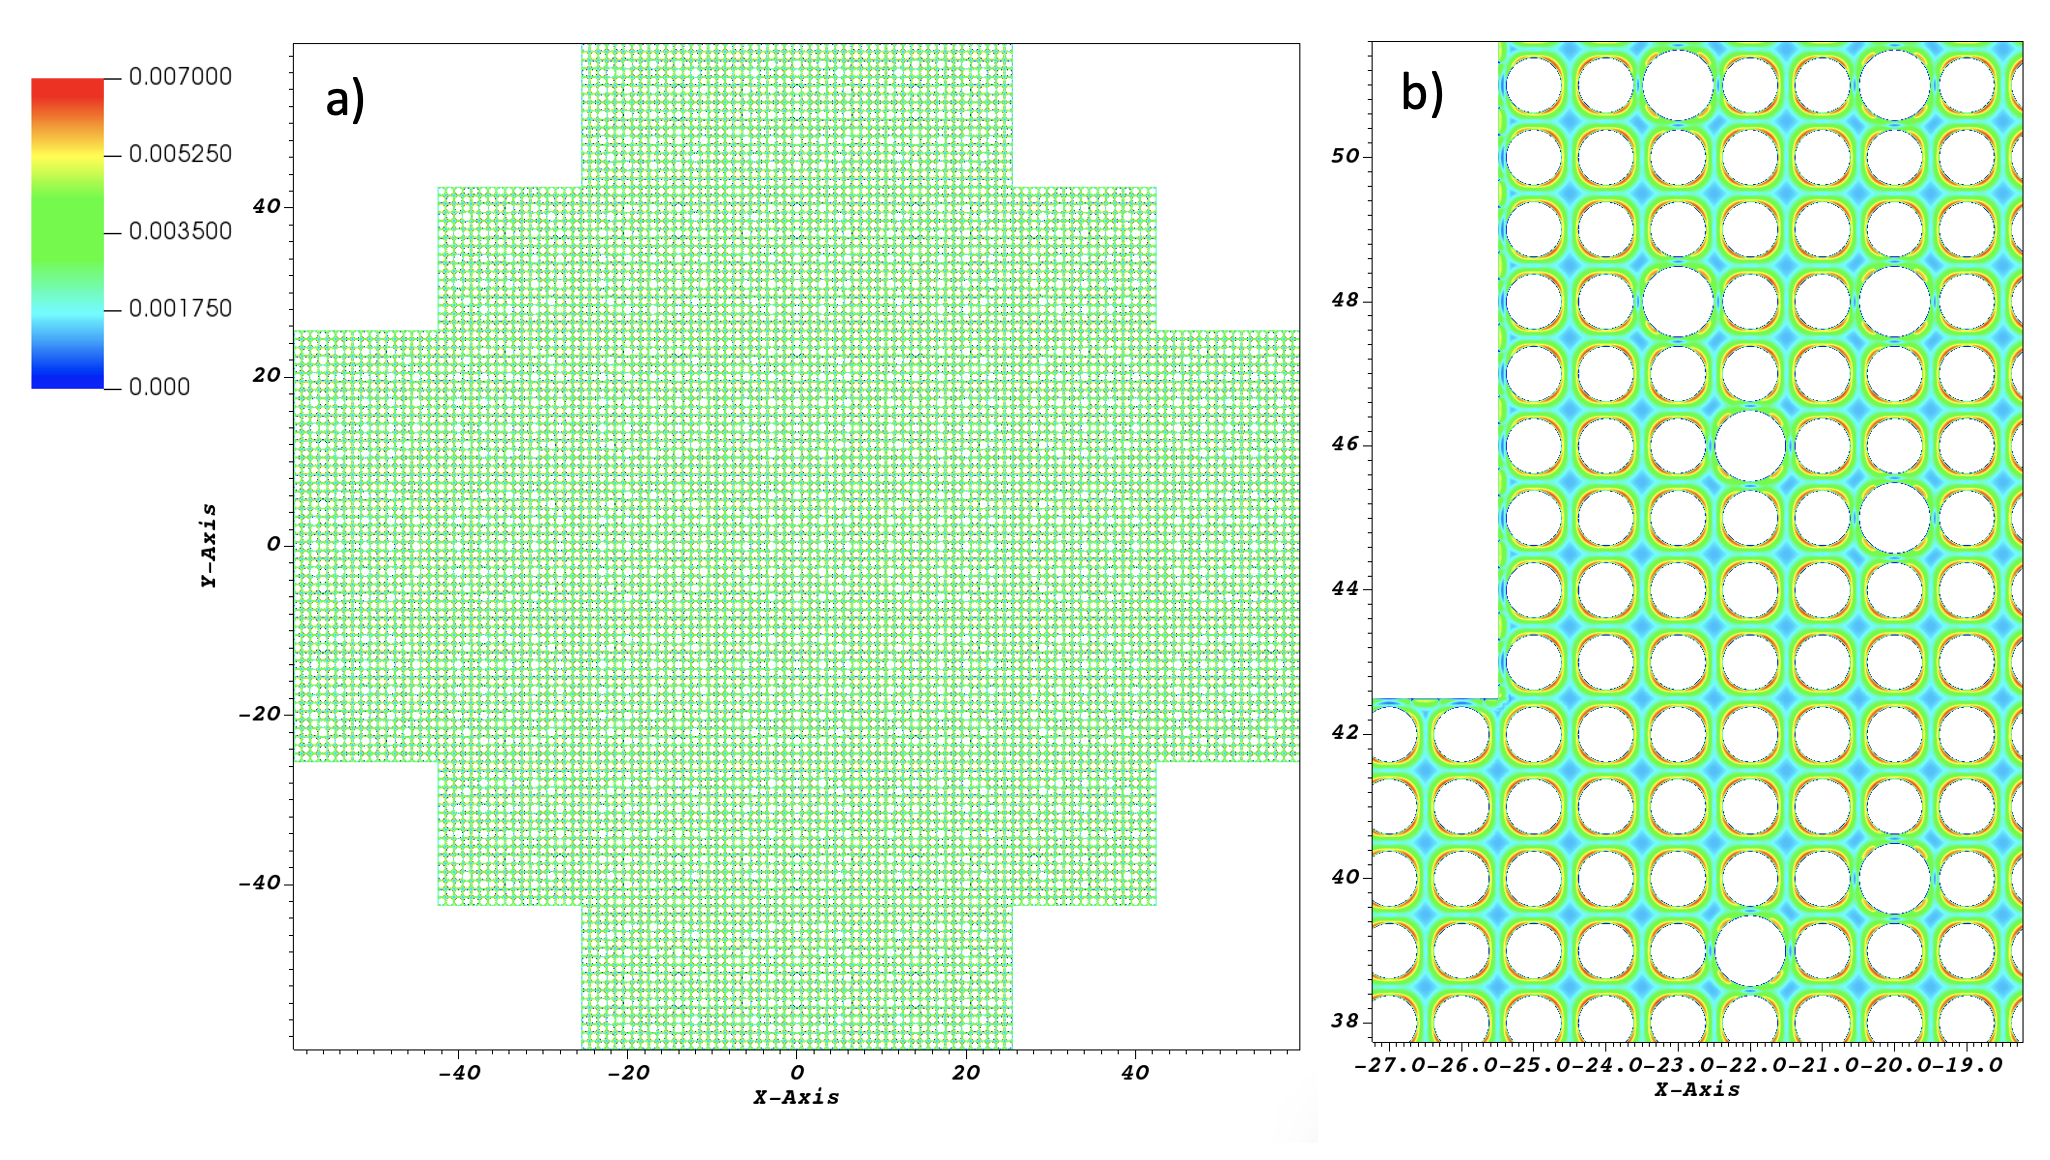
\includegraphics[width=0.9\textwidth]{./figures/periodic_tke.png}
\caption{Full core strong scaling study. a) average wall time per step. b) time per time step as simulation progresses. }
\label{fig:tke}
\end{figure}


\subsection{RANS full core simulations with momentum sources}
\label{sec:results3}

\subsection{Conjugate heat transfer}
\label{sec:results4}
